%%
%% PollingLab (c) 2021 Christopher A. Bohn
%%

%%
%% (c) 2021 Christopher A. Bohn
%%

\documentclass[12pt]{article}

\usepackage{fullpage}
\usepackage{fancyhdr}
\usepackage[procnames]{listings}
\usepackage{hyperref}
\usepackage{textcomp}
\usepackage{bold-extra}
\usepackage[dvipsnames]{xcolor}
\usepackage{etoolbox}


% Customize the semester (or quarter) and the course number

\newcommand{\courseterm}{Spring 2022}
\newcommand{\coursenumber}{CSCE 231}

% Customize how a typical lab will be managed;
% you can always use \renewcommand for one-offs

\newcommand{\runtimeenvironment}{your account on the \textit{csce.unl.edu} Linux server}
\newcommand{\filesource}{Canvas or {\footnotesize$\sim$}cse231 on \textit{csce.unl.edu}}
\newcommand{\filesubmission}{Canvas}

% These are placeholder commands and will be renewed in each lab

\newcommand{\labnumber}{}
\newcommand{\labname}{Lab \labnumber\ Assignment}
\newcommand{\shortlabname}{}
\newcommand{\duedate}{}

% Individual or team effort

\newcommand{\individualeffort}{This is an individual-effort project. You may discuss concepts and syntax with other students, but you may discuss solutions only with the professor and the TAs. Sharing code with or copying code from another student or the internet is prohibited.}
\newcommand{\teameffort}{This is a team-effort project. You may discuss concepts and syntax with other students, but you may discuss solutions only with your assigned partner(s), the professor, and the TAs. Sharing code with or copying code from a student who is not on your team, or from the internet, is prohibited.}
\newcommand{\freecollaboration}{In addition to the professor and the TAs, you may freely seek help on this assignment from other students.}
\newcommand{\collaborationrules}{}

% Do you care about software engineering?

\providebool{allowspaghetticode}

\setbool{allowspaghetticode}{false}

\newcommand{\softwareengineeringfrontmatter}{
    \ifboolexpe{not bool{allowspaghetticode}}{
        \section*{No Spaghetti Code Allowed}
        In the interest of keeping your code readable, you may \textit{not} use
        any \lstinline{goto} statements, nor may you use any \lstinline{break}
        statements to exit from a loop, nor may you have any functions
        \lstinline{return} from within a loop.
    }{}
}

\newcommand{\spaghetticodepenalties}[1]{
    \ifboolexpe{not bool{allowspaghetticode}}{
        \penaltyitem{1}{for each \lstinline{goto} statement, \lstinline{break}
            statement used to exit from a loop, or \lstinline{return} statement
            that occurs within a loop.}
    }{}
}

% You shouldn't need to customize these,
% but you can if you like

\lstset{language=C, tabsize=4, upquote=true, basicstyle=\ttfamily}
\newcommand{\function}[1]{\textbf{\lstinline{#1}}}
\setlength{\headsep}{0.7cm}
\hypersetup{colorlinks=true}

\newcommand{\startdocument}{
    \pagestyle{fancy}
    \fancyhf{}
    \lhead{\coursenumber}
    \chead{\ Lab \labnumber: \labname}
    \rhead{\courseterm}
    \cfoot{\shortlabname-\thepage}

	\begin{document}
	\title{\ Lab \labnumber}
	\author{\labname}
	\date{Due: \duedate}
	\maketitle

    \textit{\collaborationrules}
}

\newcommand{\rubricitem}[2]{\item[\underline{\hspace{1cm}} +#1] #2}
\newcommand{\bonusitem}[2]{\item[\underline{\hspace{1cm}} Bonus +#1] #2}
\newcommand{\penaltyitem}[2]{\item[\underline{\hspace{1cm}} -#1] #2}

%\usepackage{enumitem}
\usepackage{graphicx}
%\usepackage{media9}
\usepackage{addfont}
\addfont{OT1}{d7seg}{\dviiseg}
% \addfont{OT1}{deseg}{\deseg}
%\usepackage[normalem]{ulem}
%\usepackage{subfig}
\usepackage{wrapfig}
%\usepackage{animate}
\usepackage{multicol}

\renewcommand{\labnumber}{9}
\renewcommand{\labname}{Using Polling with Memory-Mapped Input/Output}
\renewcommand{\shortlabname}{memory-mapped i/o -- pollinglab}
\renewcommand{\collaborationrules}{\individualeffort}
%\renewcommand{\duedate}{soon}
\renewcommand{\duedate}{Before the start of your lab section on November 10, 15, or 16}
\newcommand{\nano}{Arduino Nano}
\renewcommand{\runtimeenvironment}{your \nano-based class hardware kit}

\startdocument

In this assignment, you will write functions to use the input and output
devices on \runtimeenvironment. You will then use those functions to implement
a number-base conversion tool using polling.

\begin{figure}[h]
    \centering
    \includegraphics[width=10cm]{AreWeThereYet}
    \caption{Polling. \tiny Image by 20th Century Fox Television}
\end{figure}

The instructions are written assuming you will edit the code in the Arduino IDE
and run it on \runtimeenvironment, constructed according to the pre-lab
instructions. If you wish, you may edit the code in a different environment;
however, our ability to provide support for problems with other IDEs is limited.

Please familiarize yourself with the entire assignment before beginning.
Section~\ref{sec:FunctionalSpecification} has the functional specification of
the system you will develop. Section~\ref{sec:Constraints} describes
implementation constraints. Section~\ref{sec:DemonstrationMode} guides you in
implementing the first portion of the system, and
Section~\ref{sec:ConversionMode} offers suggestions in implementing the second
portion of the system.

\section{Number-Base Conversion Tool Specification} \label{sec:FunctionalSpecification}

\begin{enumerate}
\item The tool shall have two modes, \textit{demonstration mode} and
    \textit{conversion mode}.
\item When the \textbf{left switch} is toggled to the left, the tool is in
    demonstration mode. When the tool is in demonstration mode:
    \begin{enumerate}
    \item \label{spec:illuminateLED} Whenever the user presses a button on the
        \textbf{matrix keypad}, the \textbf{external LED} shall illuminate for
        approximately one-half of a second.
    \item The \textbf{external LED} shall not illuminate except as specified in
        requirement~\ref{spec:illuminateLED}.
    \item Initially, no digits on the \textbf{7-segment display module} shall
        have any of their segments illuminated.
    \item Whenever the user presses a button on the \textbf{matrix keypad}, the
        corresponding hexadecimal digit shall be displayed in the
        least-significant digit position of the \textbf{7-segment display
        module}, replacing any digit previously displayed.
    \end{enumerate}
\item \label{spec:ConversionMode} When the \textbf{left switch} is toggled to
    the right, the tool is in conversion mode. When the tool is in conversion
    mode:
    \begin{enumerate}
    \item The tool shall have two sub-modes, \textit{decimal} and
    \textit{hexadecimal}.
    \item When the \textbf{right switch} is toggled to the left, the tool is in
         decimal sub-mode. When the \textbf{right switch} is toggled to the
        right, the tool is in hexadecimal sub-mode.
    \item Initially, no digits on the \textbf{7-segment display module} shall
        have any of their segments illuminated.
    \item \label{spec:BuildingValue} Whenever the user presses a button on the
        \textbf{matrix keypad}, the corresponding digit shall be displayed in
        the least-significant position of the \textbf{7-segment display
        module}, and any digits already displayed shall increase in
        significance by one order of magnitude. For example, if {\dviiseg 234}
        is displayed and the user presses \texttt{5} then {\dviiseg 2345} shall
        be displayed.
        \begin{enumerate}
        \item If the tool is in hexadecimal sub-mode, hexadecimal digits shall
            be displayed.
        \item ``0x'' shall not be displayed as part of a hexadecimal value.
        \item If the tool is in decimal sub-mode, decimal digits shall be
            displayed. If the user had pressed one of the \textit{A-F} buttons,
            it shall be ignored.
        \item If a negative decimal value is displayed, the negative sign shall
            be displayed immediately to the left of the most-significant digit
            being displayed. For example, {\dviiseg-456} is correctly
            displayed, but {\dviiseg -    456} is not correctly displayed.
        \item A positive sign shall not be displayed as part of a positive
            decimal value.
        \item Leading 0s shall not be displayed. For example, {\dviiseg 782} is
            correctly displayed, but {\dviiseg 00000782} is not correctly
            displayed.
        \item In no case shall the tool allow the user to input a value too
            great to be displayed on the \textbf{7-segment display module}. If
            the user attempts to enter a value greater than 0x7FFF,FFFF in
            hexadecimal, less than 0x8000,000 in hexadecimal, greater than
            99,999,999 in decimal, or less than -9,999,999 in decimal, then the
            \textbf{7-segment display module} shall display {\dviiseg too big}.
        \end{enumerate}
    \item Whenever the user toggles the \textbf{right switch}, the value
        previously displayed on the \textbf{7-segment display module} shall be
        re-displyed according to the new sub-mode. For example, if the tool is
        in decimal sub-mode and is displaying {\dviiseg 1234} then after the
        user changes the tool to hexidecimal sub-mode, {\dviiseg 4D2} shall be
        displayed. Similarly, if the tool is in hexadecimal sub-mode and is
        displaying {\dviiseg 1234} then after the user changes the tool to
        decimal sub-mode, {\dviiseg 4660} shall be displayed.
        \begin{enumerate}
        \item If the value is too great to be displayed in the new sub-mode,
            then {\dviiseg error} shall be displayed.
        \end{enumerate}
    \item Whenever the user presses the \textbf{left pushbutton}, the value
        being displayed shall be negated.
        \begin{enumerate}
        \item In decimal sub-mode, the presence or absence of negative sign
            shall indicate whether a value is negative or not.
        \item In hexadecimal sub-mode, 32-bit two's complement shall be used.
        \end{enumerate}
    \end{enumerate}
    \item Regardless of mode, whenever the user presses the \textbf{right
        pushbutton}, the \textbf{7-segment display module} shall be cleared. If
        the system is in conversion mode then pressing the \textbf{right
        pushbutton} will also clear the value.
    \item When the user presses a button for less than approximately one-half of a second, regardless of whether it is one of the \textbf{pushbuttons} or a button on the \textbf{matrix keypad}, it shall be treated as a single button press.
\end{enumerate}

\section{Constraints}\label{sec:Constraints}

All input and output must be accomplished using the memory-mapped I/O
registers. You may use any constants, arrays, structs, typedefs, or macros
present in the \textit{cowpi.h} header file provided as part of this
assignment. You may use any code that you write yourself. You may use any
features that are part of the C standard if they are supported by the
compiler. Except as noted below, you may \textit{not} use any libraries,
functions, macros, types, or constants that are part of the Arduino
core\footnote{\url{https://www.arduino.cc/reference/en/}} (unless they are
also part of the C standard), nor AVR-specific functions, macros, types, or
constants of avr-libc\footnote{\url{https://www.nongnu.org/avr-libc/user-manual/index.html}}.

You \textit{may} use the
\function{millis()}\footnote{\url{https://www.arduino.cc/reference/en/language/functions/time/millis/}}
function to measure the passage of time, and you \textit{may} use the
\function{Serial.begin()}\footnote{\url{https://www.arduino.cc/reference/en/language/functions/communication/serial/begin/}},
\function{Serial.print()}\footnote{\url{https://www.arduino.cc/reference/en/language/functions/communication/serial/print/}}, and
\function{Serial.println()}\footnote{\url{https://www.arduino.cc/reference/en/language/functions/communication/serial/println/}} functions for debugging.

(A quick note on using \function{print()} and \function{println()} for
debugging: if you print too much, the UART buffer may fill, making it
difficult to upload a new program to the \nano. If you have an upload
failure in this situation, the simplest fix in this case is to unplug the
\nano, plug it back in, and re-attempt the upload.)

\section{Implementing Demonstration Mode} \label{sec:DemonstrationMode}

You will use ``demonstration mode'' to configure your \nano\ to use the
memory-mapped input/output controls and peripheral devices.

\subsection{Simple Input/Output}

The ATmega328 microcontroller\footnote{\url{http://ww1.microchip.com/downloads/en/DeviceDoc/Atmel-7810-Automotive-Microcontrollers-ATmega328P_Datasheet.pdf}}
on the \nano\ has three input/output ports accessible by external pins. Each
port has three registers, the PIN input register, the PORT output register, and
the DDR data direction register used to set each pin as input or output. Each
pin is individually controlled by a particular bit in the port registers.
Figure~\ref{fig:IoPortRegisters} shows these nine registers and their
corresponding addresses, and Table~\ref{table:DataDirection} shows how to
configure the specific pins.

\begin{figure}
    \centering
    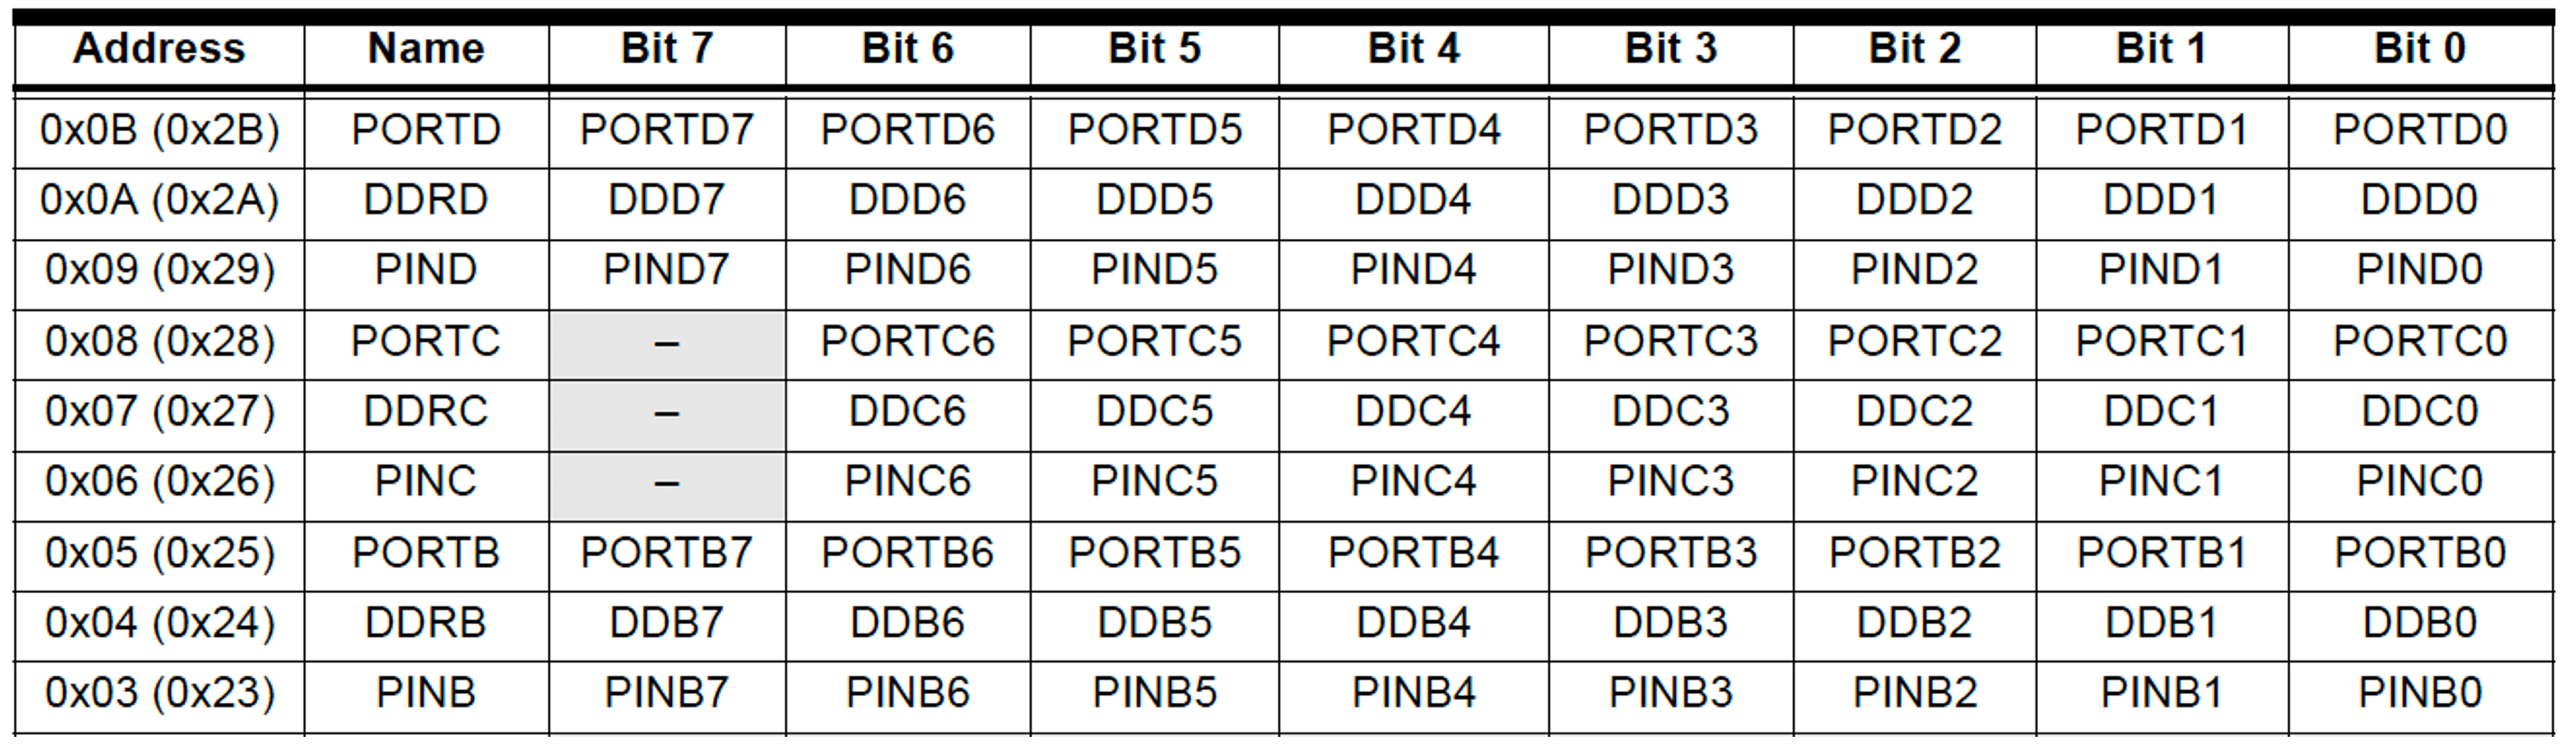
\includegraphics[width=15cm]{IoPortRegisters}
    \caption{ATmega328 I/O port registers. \tiny Cropped from ATmega382P Data Sheet, §30 \label{fig:IoPortRegisters}}
\end{figure}

\begin{table}
    \centering
    \begin{tabular}{|c|c|c|l|}
        \hline
        \textbf{DDx\textit{n}} & \textbf{PORTx\textit{n}} & \textbf{Direction} & \textbf{High/Low Value} \\ \hline \hline
        0 & 0   & Input, Hi-Z       & Takes on value from input device \\
        0 & 1   & Input, Pull-Up    & High unless input device pulls value low \\
        1 & 0/1 & Output            & Value assigned by program \\ \hline
    \end{tabular}
    \caption{Configuring I/O port pins. \tiny Adapted from ATmega382P Data Sheet, Table~13-1. \label{table:DataDirection}}
\end{table}

Figure~\ref{fig:NanoPinMapping} shows which bit in which port corresponds to
each \nano\ pin. For example, pin \texttt{D10} is labeled ``PB2'' indicating
that it is part of port B and uses bit 2 in each of port B's registers. If we
wish to use \texttt{D10} as an output pin, then we would set register
\texttt{DDRB}'s bit 2 to a 1 in our \function{setup()} function, and then our
\function{loop()} function (or other functions it calls) would set register
\texttt{PORTB}'s bit 2 to a 0 or 1 as needed, based on which logic level is
needed by the output device.

\begin{figure}
    \centering
    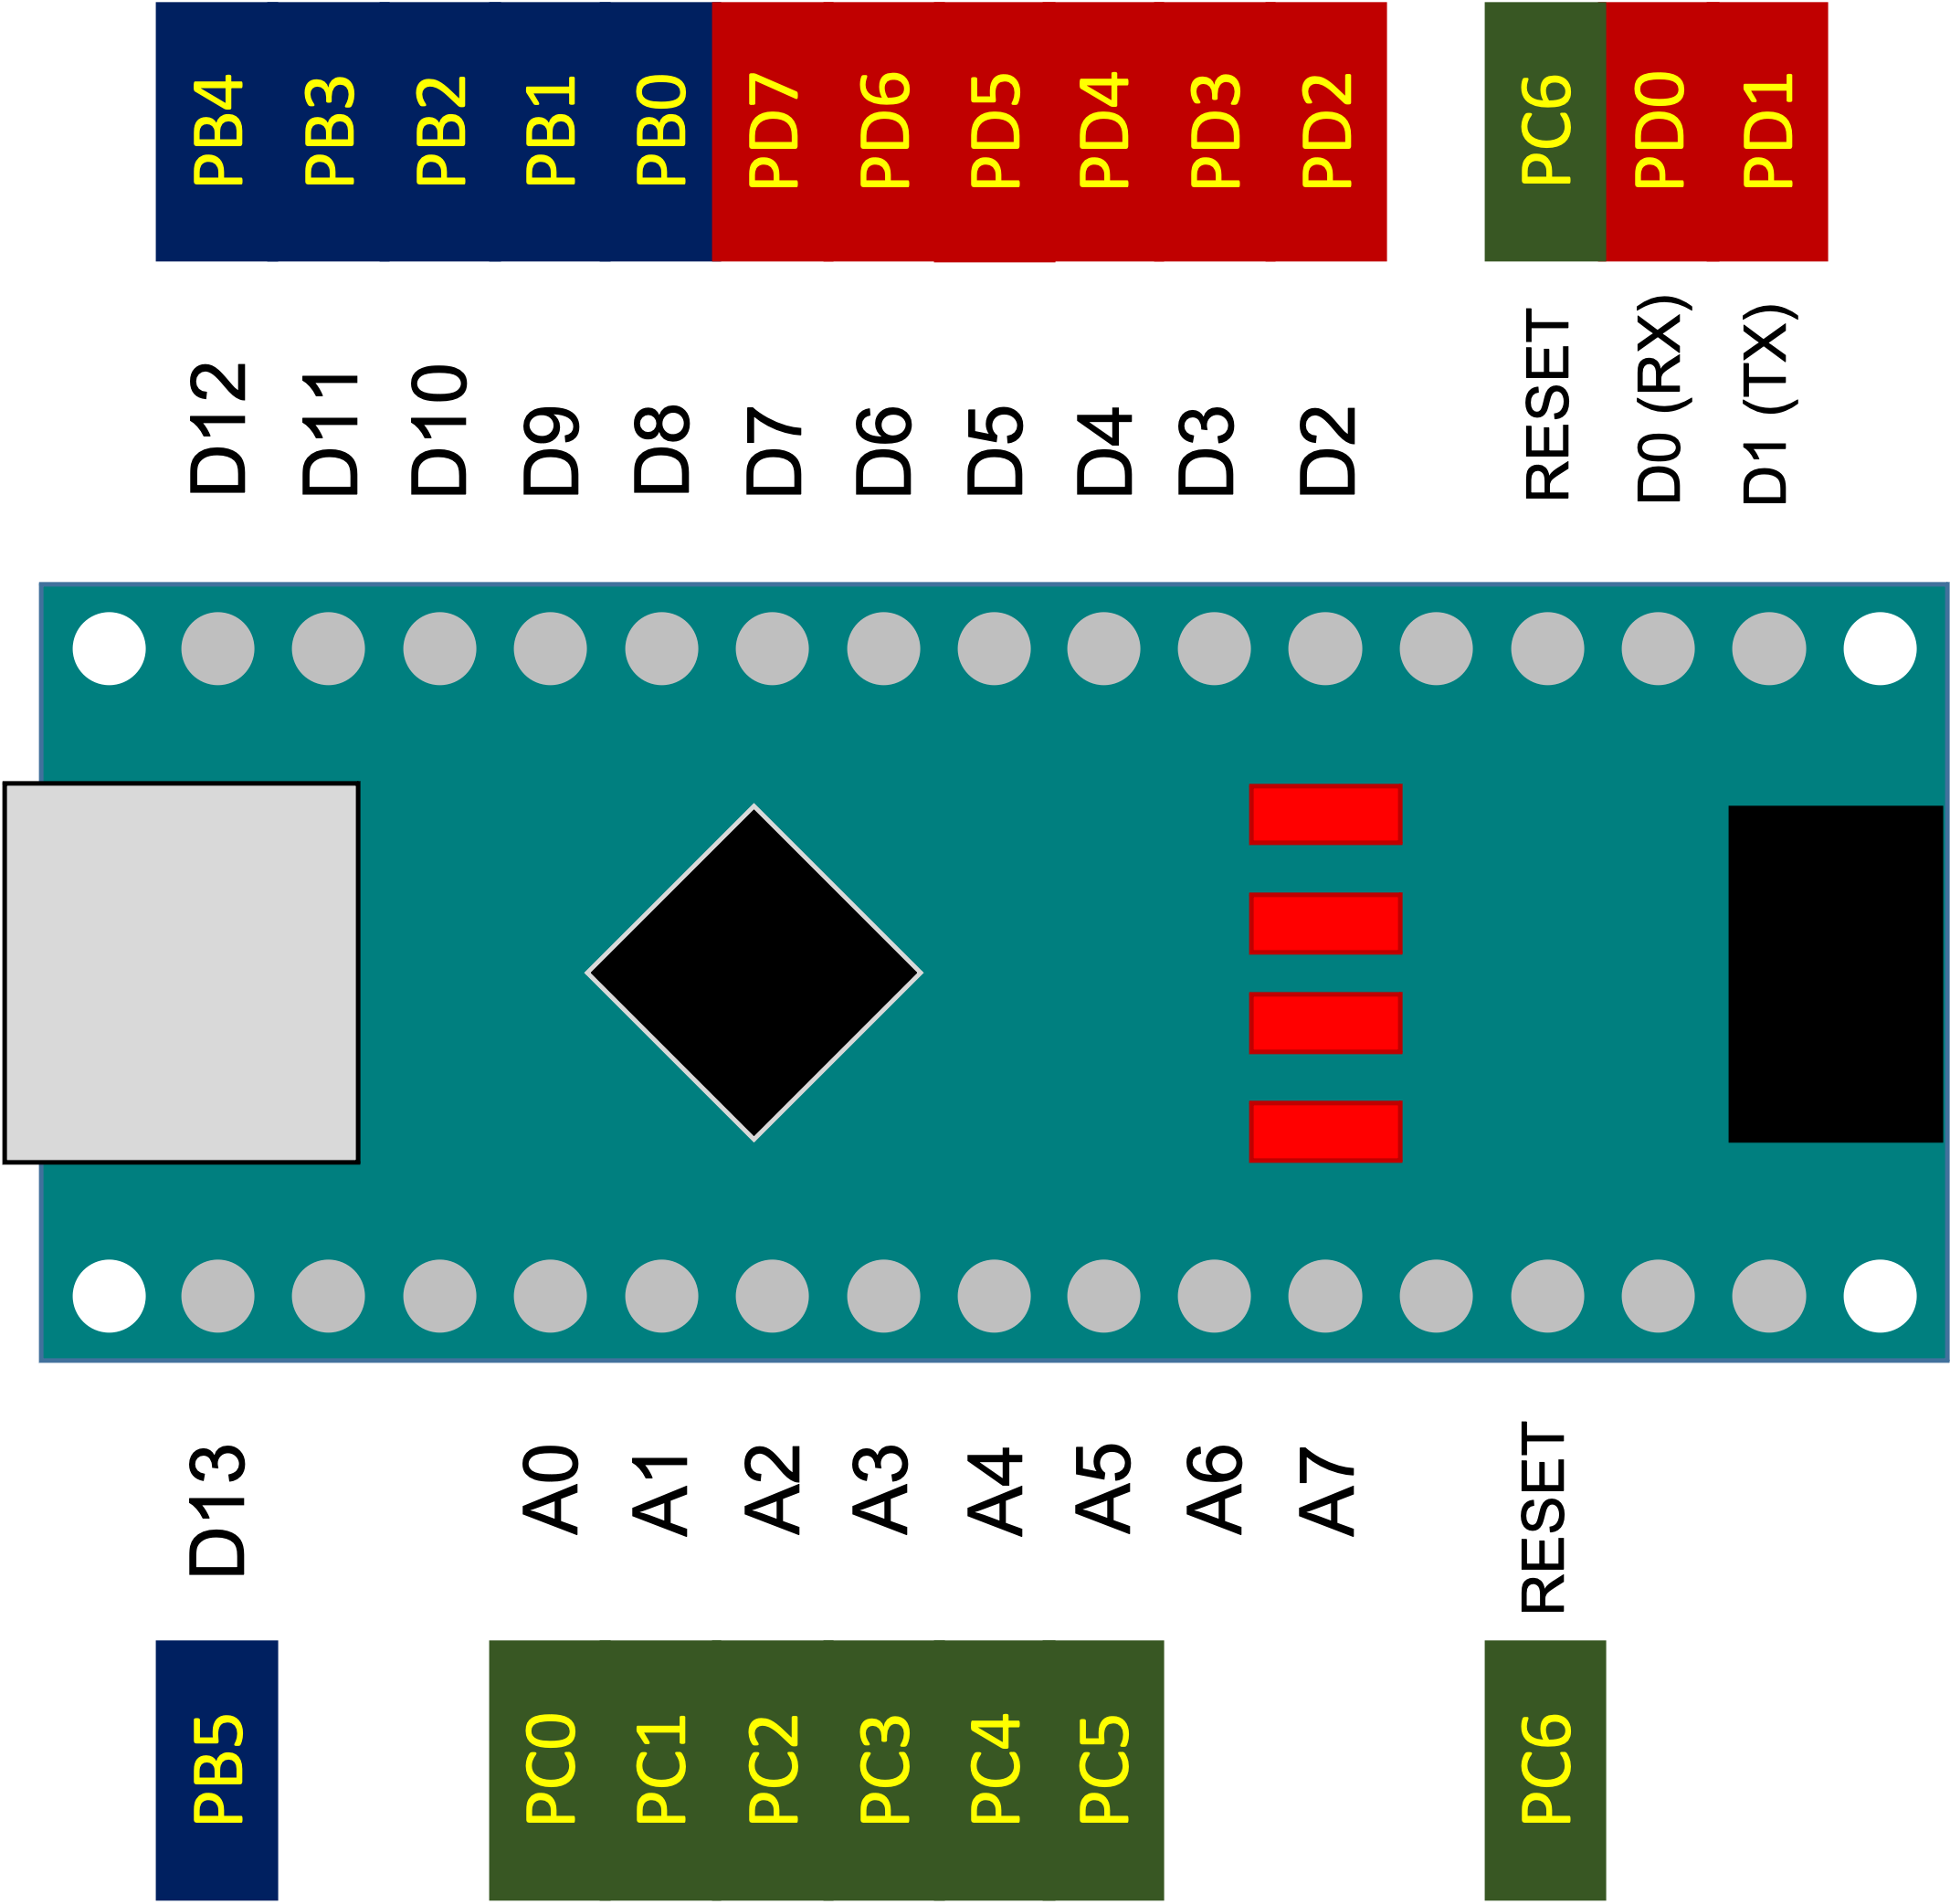
\includegraphics[width=10cm]{NanoPinMapping}
    \caption{Mapping of \nano\ pins to ATmega328 input/output ports. \tiny Diagram by Bohn \label{fig:NanoPinMapping}}
\end{figure}

On the other hand, if we wanted to use \texttt{D10} as an input pin, then we
would set register \texttt{DDRB}'s bit 2 to a 0 in our \function{setup()}
function. If we wanted the logic value to be whichever logic value is set by
the input device then we would place the pin in a ``high-impedance'' state by
setting \texttt{PORTB}'s bit 2 to 0. (Note that if the pin is in high-impedance
input mode and a logic value is not being set by an input device, the pin's
value will ``float'' and will change at the whims of stray electrons.) If we
wanted the logic level to normally be high but can be pulled low when an input
device grounds the pin, then we would set \texttt{PORTB}'s bit 2 to 1, and an
internal pull-up resistor will prevent a short circuit. You would use high-
impedance input mode when the input device is able to set both high and low
values, such as with a dual-throw switch or an active input device; you would
use pull-up input mode when the input device is able to set only one value,
such as with a single-throw switch or button.

\subsubsection{Accessing I/O Registers}

Open \textit{PollingLab.ino} in the Arduino IDE. There is a global variable,
\lstinline{gpio}, that you will use to access the input/output registers for
the external pins. If you look in \textit{cowpi.h}, you will see a constant
pointer, \lstinline{IObase} that holds the memory address that is the start of
ATmega328's memory-mapped input/output register bank. On line 10, you will see
a comment noting that the external pins' input/output registers start 3 bytes
above \lstinline{IObase}.

    \begin{itemize}
    \item On line 43 of \textit{PollingLab.ino}, find this line in \function{setup}: \lstinline{// gpio = ...}
    \item Remove the comment mark and ellipses, and assign to \lstinline{gpio} the address 3 bytes above \lstinline{IObase}.
    \end{itemize}

You can now use \lstinline{gpio} as a 3-element array to access each of the
three I/O ports. Notice in \textit{cowpi.h} there are three constants defined
to allow you index this array without having to remember which I/O port
corresponds to which set of external pins. Each element of the \lstinline{gpio}
array is a \lstinline{struct gpio_registers} with three fields:
\lstinline{input}, \lstinline{output}, and \lstinline{direction}, corresponding
to the \texttt{PINx}, \texttt{PORTx}, and \texttt{DDRx} registers, respectively.

    \begin{itemize}
    \item Recall that the left switch is connected to pin \texttt{A4} and the
        right switch is connected to pin \texttt{A5}.
    \item In the \function{setup_simple_io()} function in
        \textit{PollingLab.ino}, use the \lstinline{gpio} array to set pins
        \texttt{A4} and \texttt{A5} to \textbf{high-impedance input}. Refer to
        Figures~\ref{fig:IoPortRegisters} and/or \ref{fig:NanoPinMapping} to
        determine which bits needs to be set. Use
        Table~\ref{table:DataDirection} to determine which values those bits
        need to be set to. \textbf{\textit{Take care not to change bits that
        you don't need to change.}}
    \item Recall that the left pushbutton is connected to pin \texttt{D8} and
        the right pushbutton is connected to pin \texttt{D9}.
    \item In \function{setup_simple_io()}, use the \lstinline{gpio} array to
        set pins \texttt{D8} and \texttt{D9} to \textbf{pulled-up input}.
    \item Recall that the external LED is connected to pin \texttt{D12} thorugh
        a current-limiting resistor.
    \item In \function{setup_simple_io()}, use the \lstinline{gpio} array to
        set pins \texttt{D12} to \textbf{output}.
    \end{itemize}

\subsubsection{Testing Your Configuration}

The starter code includes a \function{test_simple_io()} function. If you upload
\textit{PollingLab.ino} to your \nano, you will see on the Serial Monitor a
message whenever you press a button or toggle a switch. The external LED will
also light up whenever both switches are in the right position (if the room is
bright, you may have to shade the LED with your hand to see that it has
illuminated). You can use this function to check whether you wrote
\function{setup_simple_io()} correctly.

You may notice the code comparing \lstinline{now} with the time a button or
switch was last used and acting only if at least 500ms have passed. This serves
two purposes.
\begin{description}
\item [Debouncing] Mechanical buttons and switches demonstrate a phenomenon
    called \textit{switch bounce}. This causes voltage to fluctuate for
    hundreds of microseconds when the contacts close or open. When this
    fluctuation is in the indeterminate region between the logical low and high
    thresholds, it can cause the logic level to ``bounce'' back-and-forth
    between high and low until settling into the final, correct logic level.
    This causes the digital circuitry or software to ``see'' multiple
    triggering events. \\
    \begin{itemize}
    \item The traditional way to debounce is to introduce a simple low-
    pass filter using a resistor and a capacitor. Hardware design can be
    simplified by solving a hardware problem with software, and so you will
    often see hobby projects with ``debouncing code'' such as
    \lstinline{delay(2);} that pauses execution between detecting the first
    change of the button's or switch's position and acting upon it for 2ms,
    ample time for switch bounce to stabilize. The problem (beyond
    \lstinline{delay()} being disallowed in this lab) is that
    2,000µs is a long time to leave your system completely non-responsive.
    \item The solution used here allows your system to continue to respond to
    other external events. For example, you can press both buttons at very
    nearly the same time (or, unlikely, at the exact same time) and the
    software will react to both immediately.
    \end{itemize}
\item [Detecting single presses] If we did nothing, then when we pressed a
    button, the code that detects the button press would see the low logic
    value every time \function{loop()} iterated, causing the message to print
    repeatedly until we lifted our finger. The solution used here allows a
    momentary press of a button to be treated as a single event but also allows
    the user to hold the button down and have the software recognize that the
    user has been holding it down longer.
\end{description}

\subsubsection{Replacing Disallowed Function Calls}

The \function{test_simple_io()} function uses \function{digitalRead()} and
\function{digitalWrite()}, two functions that are part of the Arudino core that
you cannot use in this lab. After you've satisfied yourself that you correctly
configured pins \texttt{A4}, \texttt{A5}, \texttt{D8}, \texttt{D9}, and
\texttt{D12}, you need to remove these functions.

    \begin{itemize}
    \item Use the \lstinline{gpio} array to read from \texttt{A4}, \texttt{A5},
        \texttt{D8}, and \texttt{D9} instead of using \function{digitalRead()}.
        Confirm that \function{test_simple_io()} functions the same.
    \item Now use the \lstinline{gpio} array to write to \texttt{D12} instead of
        using \function{digitalWrite()}.Confirm that \function{test_simple_io()}
        functions the same.
    \end{itemize}

\subsection{Matrix Keypad}

\begin{wrapfigure}{r}{0.3\textwidth}
    \centering
    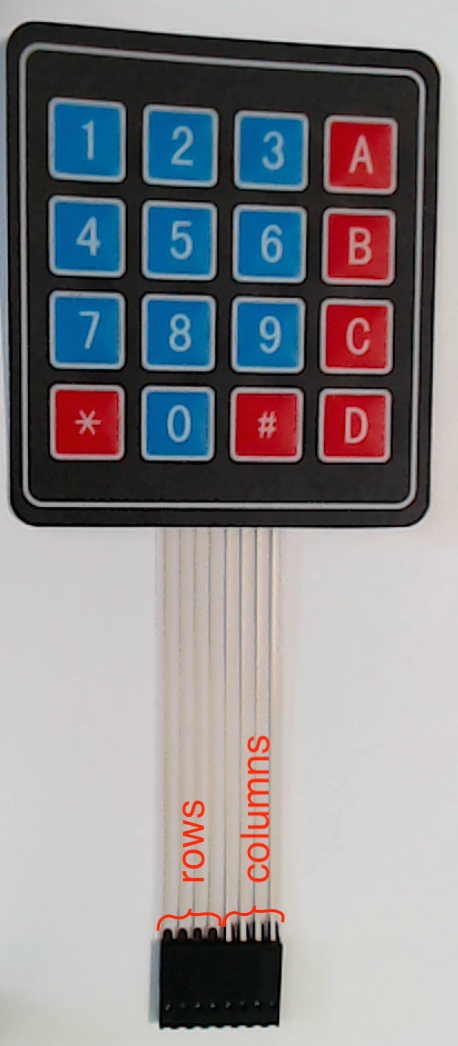
\includegraphics[width=0.25\textwidth]{keypad-annotated}
    \caption{The numeric keypad's header has four row pins and four column pins. \tiny Photograph and annotations by Bohn \label{fig:keypad-annotated}}
\end{wrapfigure}

The matrix keypad has sixteen buttons but connects only to eight pins. Instead
of reading the button presses directly, we scan the matrix to determine
which row and which column the pressed button is in. We do this by setting
logic levels on the rows and reading logic levels on the columns.

    \begin{itemize}
    \item Recall that \texttt{row1} is connected to \texttt{D4}, \texttt{row4}
        pin to \texttt{D5}, \texttt{row7} to \texttt{D6}, and \texttt{row*} to
        \texttt{D7}.
    \item In the \function{setup_keypad()} function, use the \lstinline{gpio}
        array to set pins \texttt{D4}, \texttt{D5}, \texttt{D6}, and
        \texttt{D7} to \textbf{output}. Refer to
        Figures~\ref{fig:IoPortRegisters} and/or \ref{fig:NanoPinMapping} to
        determine which bits needs to be set. Use
        Table~\ref{table:DataDirection} to determine which values those bits
        need to be set to. \textbf{\textit{Take care not to change bits that
        you don't need to change.}}
    \item In the \function{setup_keypad()} function, use the \lstinline{gpio}
        array to set the initial output values of \texttt{D4}, \texttt{D5},
        \texttt{D6}, and \texttt{D7} to 0.
    \item Recall that \texttt{column1} is connected to \texttt{A0},
        \texttt{column2} pin to \texttt{A1}, \texttt{column3} to \texttt{A2},
        and \texttt{columnA} to \texttt{A3}.
    \item In \function{setup_keypad()}, use the \lstinline{gpio} array to
        set pins \texttt{A0}, \texttt{A1}, \texttt{A2}, and \texttt{A3} to
        \textbf{pulled-up input}.
    \end{itemize}

\subsubsection{Scanning the Keypad}

There are a few options for obtaining the value corresponding to a key that is
pressed on the keypad. The most efficient for a simple application such as the
Conversion Tool is to use a lookup table. Starting on line 24 of
\textit{PollingLab.ino} you will find a 2-dimensional array that will serve as
the lookup table. The element \lstinline{keys[0][0]} will correspond to the
\texttt{1} key; \lstinline{keys[0][3]} will correspond to the \texttt{A} key;
\lstinline{keys[3][0]} will correspond to the \texttt{*} key; and
\lstinline{keys[3][3]} will correspond to the \texttt{D} key.

We want the numerals \texttt{0}-\texttt{9} to produce their respective decimal
(and hexadecimal) values. We want \texttt{A}-\texttt{D} to produce their
respective hexadecimal values. We want \texttt{\#} to produce the hexadecimal
value 0xE, and we want \texttt{*} to produce the hexadecimal value 0xF.

    \begin{itemize}
    \item Populate \lstinline{keys}' nested array initializer so that the
        lookup table will produce the correct value for each row/column
        combination.
    \end{itemize}

The first step in reading a value from the keypad is determining whether a key
has been pressed. If no key has been pressed, then column pins \texttt{A0}-
\texttt{A3} will all have the value 1 because you configured the pins to pull
their logic values high when nothing forces them low. When a button is pressed,
the button's column will be electrically connected to the button's row. Since
you configured row pins \texttt{D4}-\texttt{D7} to initially hold the value 0,
this will cause the button's column pin to take on the value 0. Thus, checking
whether \textit{any} button has been pressed can be accomplished by polling
pins \texttt{A0}-\texttt{A3} to determine if each holds the value 1 or if at
least one of them holds the value 0.

    \begin{itemize}
    \item Find the \lstinline{if} block starging on line 52 in
        \textit{PollingLab.ino}. Un-comment this \lstinline{if} block.
    \item Replace the \lstinline{...} on line 52 with a conditional expression
        that evaluates to \texttt{true} whenever at least one of the column
        pins holds the value 0.
    \end{itemize}

Now locate \function{get_key_pressed()}. Notice that it has timing code similar
to what you saw in \function{test_simple_io()} that will treat a keypress that
lasts less than 500ms as a single keypress.

    \begin{itemize}
    \item Inside the \lstinline{if} block, add a \lstinline{for} loop that
        iterates over the four rows.
    \item At the start of the loop body, set each row pin to output 1, except
        that the pin corresponding to the current iteration's row should output
        0. For example, in the first iteration, you want \texttt{D5},
        \texttt{D6}, and \texttt{D7} to output a 1 but \texttt{D4} to output a
        0. You will probably find it easier to do this in two lines, first
        setting \textit{all} of the row pins to 1 and then setting the current
        iteration's row pin to 0.
    \item Poll the column pins. If all column pins are still 1, then the key
        being pressed is not in the current iteration's row. On the other
        hand\dots
    \item If one of the column pins is 0, then the key being pressed is in the
        current iteration's row. If this is the case, then determine which
        column the key is in based on which column pin is has the value 0.
    \item Knowing the key's row and column, use the lookup table to assign the correct value to the variable \lstinline{key_pressed}.
        \begin{itemize}
        \item In case you make a mistake when writing this code, you may wish
            to add error-handling code to make sure you do not make an
            assignment to \lstinline{keys_pressed} when you shouldn't have done
            so.
        \end{itemize}
    \item After the \lstinline{for} loop termintes, set the row pins back to 0.
    \end{itemize}

This design does \textit{not} handle the case of the user pressing multiple
keys simultaneously. Handling multiple simultaneous keypresses is a
considerably more-challenging problem.

\subsubsection{Testing Your Implementation}

If you implemented the keypad code correctly, then after you upload
\textit{PollingLab.ino} to your \nano, you will see on the Serial Monitor a
message with the key value whenever you press a key on the keypad. If it does
not, examine your code for errors. Adding debugging
\lstinline{Serial.print()}/\lstinline{Serial.println()} statements may help.

\subsection{7-Segment Display Module}

The 7-Segment Display Module consists of a
MAX7219\footnote{\url{https://datasheets.maximintegrated.com/en/ds/MAX7219-MAX7221.pdf}}
integrated circuit that acts as a peripheral using the SPI protocol and that
drives the eight 7-segment displays.

The \textit{Serial Parallel Interface} (SPI) is a protocol that allows data to
be sent and received serially (over a single wire) that should be used in
parallel. This protocol is common enough that the ATmega328 microcontroller
used by the \nano\ implements the protocol in hardware (see chapter 18 of the
ATmega328 datasheet).

    \begin{quote}
    NOTE: The original SPI specification used the terms \textit{MOSI} and
    \textit{MISO} to describe its two modes, and alternately used \textit{SS}
    and \textit{CS} to describe the signal that a device should listen for
    input. The preferred terminology now is \textit{COPI} (Controller Output,
    Peripheral Input), \textit{CIPO} (Controller Input, Peripheral Output) to
    describe the modes in devices that can use either mode (such as the \nano),
    \textit{SDO} and \textit{SDI} to describe the modes in devices that can
    only use one mode (the display module uses SDI), and \textit{CS} (Chip
    Select) exclusively to describe the signal indciating that a device should
    listen for input.

    We will use the preferred terminology; however, legacy documentation --
    including the ATmega328 and MAX7219 datasheets -- still use the original
    terminology.
    \end{quote}

The MAX7219 receives the serial data into a shift register and then latches the
shift register's bits in parallel into one of eight memory locations or one of
five control registers. The starter code takes care of configuring the
MAX7219's control registers. Your task will be to write the code that sends
data to the display module.

The eight memory locations in the MAX7219 each correspond to one of the eight
digits. The least-significant digit has the address 1, and the most-significant
digit has the address 8. The bit pattern in each of these addresses indicates
which LEDs in the 7-segment display should be illuminated (see
Figure~\ref{fig:SevenSegment}).

\begin{figure}
    \centering
    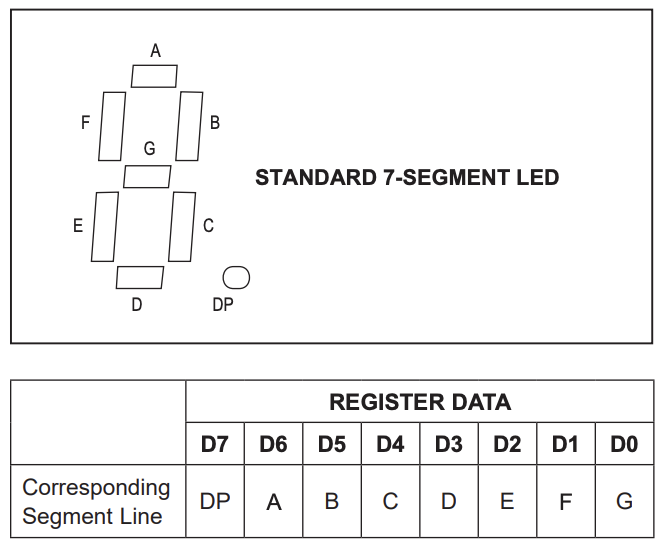
\includegraphics[width=10cm]{SevenSegment}
    \caption{Mapping of bits to 7-segment LEDs. \tiny Copied from MAX7219 Data Sheet, Table~6 \label{fig:SevenSegment}}
\end{figure}

Seven-segment displays are so-named because (not including the decimal point)
there are seven segments that can be activated/deactivated in combinations to
form the ten decimal numerals (and, with a little imagination, most of the
letters in the Latin alphabet). In the case of our display module, the segments
are LEDs; you might also see segmented displays using LCDs or flip panels.

\subsubsection{Configuring the \nano\ for SPI}

There is a global variable in \textit{PollingLab.ino},
\lstinline{spi}, that you will use to access the SPI registers for
the external pins. If you look in \textit{cowpi.h}, you will see on line 21,
you will see a comment noting that the SPI registers start 0x2C bytes above
\lstinline{IObase}.

    \begin{itemize}
    \item On line 44 of \textit{PollingLab.ino}, find this line in \function{setup}: \lstinline{// spi = ...}
    \item Remove the comment mark and ellipses, and assign to \lstinline{spi} the address 0x2C bytes above \lstinline{IObase}.
    \end{itemize}

The \lstinline{struct spi_registers} has three fields: \lstinline{control},
\lstinline{status}, and \lstinline{data}, corresponding to the \texttt{SPCR},
\texttt{SPSR}, and \texttt{SPDR} registers, respectively (see
Table~\ref{table:SPIregisters}). We need to enable SPI by setting the
\texttt{SPE} bit to 1, set the \nano\ as the controller by setting the
Controller (née MSTR) bit to 1, and set the SPI clock at 1MHz by setting the
SPR1 and SPR0 bits to 01. All remaining bits in \texttt{SPCR} should be 0.

\begin{table}
    \centering \small
    \begin{tabular}{|r||c|c|c|c|c|c|c|c||}
        \hline
        Bit                         & \textbf{7}    & \textbf{6}    & \textbf{5}    & \textbf{4}    & \textbf{3}    & \textbf{2}    & \textbf{1}    & \textbf{0}    \\ \cline{2-9} \cline{2-9}
        \textbf{SPDR} 0x2E (0x4E)   & MSB           & \dots         & \dots         & \dots         & \dots         & \dots         & \dots         & LSB           \\
        \textbf{SPSR} 0x2D (0x4D)   & SPIF          & WCOL          & not used      & not used      & not used      & not used      & not used      & SPI2X         \\
        \textbf{SPCR} 0x2C (0x4C)   & SPIE          & SPE           & DORD          & Controller    & CPOL          & CPHA          & SPR1          & SPR0          \\ \hline
    \end{tabular}
    \caption{SPI Data, Status, and Control Registers. \tiny Adapted from ATmega382P Data Sheet, §18.5. \label{table:SPIregisters}}
\end{table}

    \begin{itemize}
    \item Replace the first line in \function{setup_display_module()} that says
        \\ \phantom{sp} \lstinline{// Set COPI, SCK, and CS to output} \\ with
        code that uses the \lstinline{gpio} array to set pins \texttt{D11},
        \texttt{D13}, and \texttt{D10} to output.
    \item Replace the second line in \function{setup_display_module()} that says
        \\ \phantom{sp} \lstinline{// Enable SPI, Controller, set clock rate fck/16}
        \\ with code that uses the \lstinline{spi} struct to set the bits in
        the SPI Control Register to the desired values.
    \end{itemize}

\subsubsection{Displaying Values}

We will use a lookup table to determine the bit patterns that need to be sent
to the display module. Starting on line 35 of \textit{PollingLab.ino} you will
find a 1-dimensional array that will serve as the lookup table. The element
\lstinline{seven_segments[0]} will contain the bit pattern for the numeral
{\dviiseg 0},  \lstinline{seven_segments[1]} will contain the bit pattern for
the numeral {\dviiseg 1}, and so on through  \lstinline{seven_segments[15]}
which will contain the bit pattern for the hex numeral {\dviiseg F}. For
reference, Figure~\ref{fig:SevenSegmentNumerals} shows the desired segments
that to be activated for each of the sixteen numerals. (Clearing a digit is
achieved by sending 0x00 to that digit's corresponding memory address,
deactivating all segments for that digit. This is demonstrated in
\function{setup_display_module()}. You do not need to include this in the
lookup table.)

\begin{figure}
    \centering
    {\dviiseg \huge 0123456789ABCDEF \\ \vspace{0.1cm}
                   8888888888888888}
    \caption{Segments to be activated for the sixteen numerals. The first row shows the segments to be activated; the second row shows all segments to more clearly show which segment is which. \label{fig:SevenSegmentNumerals}}
\end{figure}

In \function{display_data()}:
    \begin{itemize}
    \item Use the \lstinline{gpio} array to set \texttt{D10} to 0, instructing
        the display module to receive data.
    \item The MAX7219 expects the address to be sent before the value. Use the
        \lstinline{spi} struct to place \lstinline{address} in the SPI Data
        Register.
    \item You should not place any new data into the SPI Data Register until
        the previous data has been sent; the \texttt{SPIF} bit in the SPI
        Status Register is a 0 when data is being sent and is a 1 when the data
        has been sent. Write a \lstinline{while} loop that does nothing except
        continue to iterate while the \texttt{SPIF} bit is a 0 (use the
        \lstinline{spi} struct to poll the SPI Status Register).
    \item Now use the \lstinline{spi} struct to place \lstinline{value} in the
        SPI Data Register.
    \item Write another \lstinline{while} loop that does nothing except
        continue to iterate while the \texttt{SPIF} bit is a 0.
    \item Use the \lstinline{gpio} array to set \texttt{D10} to 1, instructing
        the display module to latch the data into its memory.
    \end{itemize}

\subsubsection{Testing Your Implementation}

On line 57 of \textit{PollingLab.ino}, find this line in \function{loop}: \\
\lstinline{// display_data(1, seven_segments[keypress]);}. If you correctly
implemented the keypad code and the display code then any key you press on the
matrix keypad will display in the least-significant digit of the seven-segment
display module. If it does not, examine your code for errors. Adding debugging
\lstinline{Serial.print()}/\lstinline{Serial.println()} statements may help.

\subsection{Completing Demonstration Mode}

Most of the code for Demonstration Mode is now complete.

    \begin{itemize}
    \item Either remove the call to \function{test_simple_io()} in
        \function{loop()} or remove the line in \function{test_simple_io()} that
        causes the external LED to illuminate, since this is \textit{not} the
        behavior we want for the external LED.
    \item Add code to cause the external LED to illuminate when a key on the
        keypad is pressed and to deluminate 500ms later.
    \item Add code so that demonstration mode only executes when the left
        switch is in the left position.
    \item Add code so that when the system enters demonstration mode, all
        digits on the display module are cleared.
    \item Add code so that when the user presses the right pushbutton, all
        digits on the display module are cleared.
    \end{itemize}

\section{Implementing Conversion Mode} \label{sec:ConversionMode}

When the system is not in demonstration mode, it is in conversion mode. Add
code so that when the system enters conversion mode (when the left switch is
moved to the right position), all digits on the display are cleared. Add code
to the ``clearing'' code (at least to the ``clearing'' code associated with the
right pushbutton) that also clears the value being built.

The best way to tackle conversion mode is to break it into bite-sized
subproblems. Start by implementing the code to build the value in accordance
with requirement~\ref{spec:BuildingValue}. Here are some recommendations:
    \begin{itemize}
    \item Start without considering the negation button.
    \item Keep an array of the bit patterns to be displayed separate from the
        actual value being built. While it won't matter as much in hexadecimal
        sub-mode, constantly re-calculating the BCD representation of a value
        every time a key is pressed in decimal mode may become a performance
        bottleneck since division (and modulo) is not implemented in hardware
        \textit{and} even the (8-bit) hardware-implemented arithmetic will
        require several processor cycles for 32-bit arithmetic on the value.
    \item When a key is pressed, update both the value being built, the
        array of display bit patterns, and the actual display. The array can be
        updated simply by moving existing bit patterns into other positions in
        the array.
    \item Conveniently, you can also use the code to update the display array
        to detect when you need to display {\dviiseg too big} instead of making
        comparisons to the value being built.
    \end{itemize}

\begin{figure}
    \centering
    {\dviiseg \huge \begin{tabular}{r} too big  \\
                                      88888888 \\
                                         error \end{tabular}}
    \caption{Segments to be activated for error messages. The first and third rows show the segments to be activated; the second row shows all segments to more clearly show which segment is which. \label{fig:SevenSegmentError}}
\end{figure}

Now that you have that code working, add code to negate the value whenever the
left pushbutton is pressed. It is possible to quickly update the display array
without using any arithmetic other than negating the value (how this is done
differs between decimal and hexadecimal sub-modes), but if you need to re-
calculate the display array that is fine. Don't forget to update the actual
display, too.

Finally, convert between radices. When moving the right switch from the left
position to the right position, convert the displayed value from decimal to
hexadecimal. When moving the right switch from the right position to the left
position, convert the displayed value from hexadecimal to decimal. Obviously,
you will need to re-calculate the display array. Don't forget to update the
actual display, too.

\section*{Turn-in and Grading}

When you have completed this assignment, upload \textit{PollingLab.ino} to
\filesubmission.

This assignment is worth 50 points. \\

Rubric:
\begin{description}
\rubricitem{10}{Simple input/output functions correctly.}
\rubricitem{10}{Matrix keypad functions correctly.}
\rubricitem{10}{7-Segment Display Module functions correctly.}
\rubricitem{1}{System is in demonstration mode only when left switch is in left position and conversion mode when the left switch is in the right position.}
\rubricitem{1}{External LED illuminates when key is pressed and deluminates 500ms later if in Demonstration mode. (This behavior is unspecified when in Conversion mode.)}
\rubricitem{2}{All digits on the display module are cleared when the system enters demonstration mode, when the system enters conversion mode, or when the right pushbutton is pressed.}
\rubricitem{3}{Builds a value consistent with requirement~\ref{spec:BuildingValue} when in decimal sub-mode.}
\rubricitem{3}{Builds a value consistent with requirement~\ref{spec:BuildingValue} when in hexadecimal sub-mode.}
\rubricitem{1}{Negates value in decimal sub-mode when left pushbutton is pressed.}
\rubricitem{1}{Negates value in hexadecimal sub-mode when left pushbutton is pressed.}
\rubricitem{3}{Converts from decimal to hexadecimal.}
\rubricitem{3}{Converts from hexadecimal to decimal.}
\rubricitem{2}{Conversion mode errors handled correctly.}
\penaltyitem{10}{Simple input/output configuration and test function relies on code that violates the constraints in Section~\ref{sec:Constraints}.}
\penaltyitem{10}{Obtaining values from matrix keypad relies on code that violates the constraints in Section~\ref{sec:Constraints}.}
\penaltyitem{10}{Sending values to the 7-segment display module relies on code that violates the constraints in Section~\ref{sec:Constraints}.}
\penaltyitem{4}{Code associated with demonstration mode (other than that covered in the first three penalty items) relies on code that violates the constraints in Section~\ref{sec:Constraints}.}
\penaltyitem{16}{Code associated with conversion mode (other than that covered in the first three penalty items) relies on code that violates the constraints in Section~\ref{sec:Constraints}.}
\bonusitem{2}{Get assignment checked-off by TA or professor during office hours before it is due. (Cannot get both bonuses.)}
\bonusitem{1}{Get assignment checked-off by TA at \textit{start} of your scheduled lab immediately after it is due. (Cannot get both bonuses.)}
\end{description}

\section*{Lab Checkoff}

You are not required to have your assignment checked-off by a TA or the
professor. If you do not do so, then we will perform a functional check
ourselves. In the interest of making grading go faster, we are offering a small
bonus to get your assignment checked-off at the start of your scheduled lab
time immediately after it is due. Because checking off all students during lab
would take up most of the lab time, we are offering a slightly larger bonus if
you complete your assignment early and get it checked-off by a TA or the
professor during office hours.

\begin{description}
\item [[ ]] Establish that the code you are demonstrating is the code you
    submitted to to \filesubmission.
    \begin{itemize}
    \item If you are getting checked-off during lab time, show the TA that the
        file was submitted before it was due.
    \item Download the file into your PollingLab directory. If necessary,
        rename it to \textit{PollingLab.ino}.
    \end{itemize}
\item [[ ]] Upload \textit{PollingLab.ino} to your \nano.
\item [] \textbf{If you completed demonstration mode, jump ahead to
    \textit{Demonstration Mode}.} Successfully completing demonstration
    \textit{prima facie} shows that the I/O functions correctly.
\item [] \textbf{If you did not complete demonstration mode:}
\item [[ ]] Using \function{test_simple_io()}, show on the Serial Monitor that
    the left and right button presses are detected.
\item [[ ]] Using \function{test_simple_io()}, show on the Serial Monitor that
    the left and right switches' position changes are detected.
\item [[ ]] Show that the external LED illuminates when it is supposed to (in a
    bright room, you may need to shade the LED with your hand). You can do this
    either by moving both switches to the right position (using the code in
    \function{test_simple_io()}) or by showing the LED illuminate when you
    press a key on the matrix keypad (if you started working on demonstration
    mode).
\item [[ ]] Show on the Serial Monitor that key presses on the matrix keypad
    are correctly decoded.
\item [[ ]] Show on the display module that values decoded from the matrix
    keypad are displayed as the correct characters.
\item[] \textbf{\textit{Demonstration Mode}}
\item[[ ]] Place the left switch in the left position. The display module is
    blank.
\item[[ ]] Press a key on the matrix keypad. The corresponding character
    appears on the display module, and the external LED illuminates for
    approximately one-half of a second.
\item[[ ]] Press a different key on the matrix keypad. The corresponding
    character appears on the display module, and the external LED illuminates
    for approximately one-half of a second.
\item[[ ]] Press the right pushbutton. The display module blanks.
\item[[ ]] Press a key on the matrix keypad. The corresponding character
    appears on the display module, and the external LED illuminates for
    approximately one-half of a second.
\item[[ ]] Press the same key on the matrix keypad. The display module is
    unchanged (still displays the corresponding character), but the external
    LED still illuminates for approximately one-half of a second.
\item[] \textbf{\textit{Conversion Mode}}
\item[[ ]] Place the left switch in the right position. The display module
    blanks.
\item[[ ]] Press a key on the matrix keypad. The corresponding character
    appears on the display module.
\item[[ ]] Place the left switch in the left position. The display module
    blanks.
\item[[ ]] Place the left switch in the right position.
\item[[ ]] Place the right switch in the left position.
\item[[ ]] Press 2, then 3. \\
    {\dviiseg \phantom{8888888}2} \\
    {\dviiseg \phantom{888888}23}
\item[[ ]] Press B. The display is unchanged.
\item[[ ]] Press the left pushbutton, then 1. \\
    {\dviiseg -\phantom{88888}23} \\
    {\dviiseg -\phantom{8888}231}
\item[[ ]] Place the right switch in the right position. \\
    {\dviiseg FFFFFF19}
\item[[ ]] Press 0, then A. \\
    {\dviiseg FFFFF190} \\
    {\dviiseg FFFF190A}
\item[[ ]] Press the left pushbutton, then \#. \\
    {\dviiseg \phantom{8888}E6F6} \\
    {\dviiseg \phantom{888}E6F6E}
\item[[ ]] Place the right switch in the left position. \\
    {\dviiseg \phantom{88}946030}
\item[[ ]] Press 4, then 5, then 6. \\
    {\dviiseg \phantom{8}9460304} \\
    {\dviiseg 94603045} \\
    {\dviiseg \phantom{8}too big}
\item[[ ]] Press the right pushbutton. The display module blanks.
\item[[ ]] Place the right switch in the right position. The display remains
    blank.
\item[[ ]] Press 7, then 8, then 9, then C, then *, then 0, then \#, then D. \\
    {\dviiseg \phantom{8888888}7} \\
    {\dviiseg \phantom{888888}78} \\
    {\dviiseg \phantom{88888}789} \\
    {\dviiseg \phantom{8888}789C} \\
    {\dviiseg \phantom{888}789CF} \\
    {\dviiseg \phantom{88}789CF0} \\
    {\dviiseg \phantom{8}789CF0E} \\
    {\dviiseg 789CF0ED}
\item[[ ]] Place the right switch in the left position. \\
    {\dviiseg \phantom{888}Error}
\item[[ ]] Press the right pushbutton. The display module blanks.
\end{description}

This concludes the demonstration of your system's functionality. The TAs will
later examine your code for violations of the assignment's constraints.
\end{document}
